%%%%%%%%%%%%%%%%%%%%%%%%%%%%%%%%%%%%%%%%%%%%%%%%%%%%%%%%%%%%%%%%%%%%%%%%%%%%%%%
%
%    LaTeX RESEARCH PROPOSAL TEMPLATE
%
%    This document is a complete, runnable guide.
%    You can click "Preview" to see it compiled into a PDF.
%
%%%%%%%%%%%%%%%%%%%%%%%%%%%%%%%%%%%%%%%%%%%%%%%%%%%%%%%%%%%%%%%%%%%%%%%%%%%%%%%

% --- 1. DOCUMENT CLASS ---
% We'll use the 'article' class. It's clean, standard, and perfect for
% proposals. We set the default font size to 11pt and paper size to A4.
\documentclass[11pt, a4paper]{article}


% --- 2. PREAMBLE: LOADING PACKAGES & SETTINGS ---

% --- UNIVERSAL PREAMBLE BLOCK (Mandatory for compilation) ---
% 'geometry' controls the page margins.
\usepackage[a4paper, top=2.5cm, bottom=2.5cm, left=2cm, right=2cm]{geometry}

% Use standard T1 font encoding
\usepackage[T1]{fontenc}
% Use UTF-8 input encoding
\usepackage[utf8]{inputenc}
% Load babel for English
\usepackage[english]{babel}
\usepackage{graphicx}
\usepackage{parskip}
\setlength{\parskip}{1em} % Sets the space between paragraphs (e.g., 1em, 12pt, 0.5cm)
\setlength{\parindent}{1em} % Removes the first-line indent
\usepackage{tabularx}
\usepackage{booktabs}
\usepackage{amssymb}
\usepackage{tikz}
\usepackage{tikz}
\usetikzlibrary{arrows.meta, positioning, quotes, shapes.geometric} 
\usepackage{longtable}
\usepackage{array}  
\usepackage{ragged2e}

% Define the styles for our blocks
\tikzset{
  block/.style = {draw, rectangle, minimum height=3em, minimum width=4em},
  sumstyle/.style = {draw, circle, minimum size=2em}, % <-- Renamed style from 'sum'
  input/.style = {coordinate},
  output/.style = {coordinate}
}
% We are not using fontspec, so the LaTeX default (Latin Modern) will be used.
% --- END UNIVERSAL PREAMBLE BLOCK ---


% --- SMART PACKAGES (For proposal content) ---

% 'amsmath' is essential for writing any mathematical formulas.
\usepackage{amsmath}

% We will use standard paragraph indentation (the LaTeX default)
% by not including the 'parskip' package.


% --- METADATA (For the title page) ---
% We define the title, author, and date here.
% The '\\' command creates a line break.
% \textit{} makes text italic.
\title{
    Energy Based Liquid Neural Network \\ % Main title
    \vspace{0.25cm} % Optional: adds a little space
    \large % Makes the subtitle a bit smaller than the main title
    Utilizing Inherent Causality of Liquid Neural Network \\ % Subtitle part 1
    for Physics-Constrained Multi-Objective Environment % Subtitle part 2
}
\author{Abu Huzaifah bin Haji bidin \\ Faculty of Management, Science and Computing \\ Universiti Teknologi PETRONAS \\ \texttt{abu\_25002382@utp.edu.my}}
\date{
    Supervisor: Dr Nurul Aida Osman\\
    Co-supervisor: Dr Shuhaida M Shuhidan\\
    \vspace{0.5cm} % Adds a little space
    October 28, 2025 % You can still include the date
}


% --- HYPERREF (Must be the LAST package) ---
% This makes your Table of Contents and references clickable.
% 'hidelinks' removes the colored boxes around links.
\usepackage[hidelinks]{hyperref}


% --- 3. THE DOCUMENT BEGINS ---
\begin{document}

% --- CUSTOM TITLE PAGE ---
% The user specifically asked for a cover page with image placeholders.
% We use the 'titlepage' environment for this.
\begin{titlepage}
    \centering % Center all content on this page
    \vfill % Pushes content vertically

    % --- LOGO PLACEHOLDER ---
    % As per Directive A, we MUST use a \framebox placeholder.
    % We cannot use \includegraphics{logo.png} here.
    % Replace this whole \framebox block with your \includegraphics command
    % when you compile this on your own machine.
    \includegraphics[width=0.2\linewidth]{UTP_LOGO.png}
    \vspace{2cm} % Adds 2cm of vertical space

    % --- TITLE & AUTHOR ---
    % We use the metadata we defined in the preamble.
    % We need \makeatletter/\makeatother to access the
    % internal macros \@title, \@author, and \@date
    % where the content is stored.
    \makeatletter
    {\huge \bfseries \@title \par} % \bfseries makes text bold
    
    \vspace{1.5cm}
    
    {\Large \@author \par} % \Large makes text larger
    
    \vspace{1.5cm}
    
    {\Large \@date \par}
    \makeatother
    
    \vfill % Fills the remaining vertical space
    
    % --- IMAGE PLACEHOLDER ---
    % Another placeholder for a key image, as requested.
\end{titlepage}


% --- TABLE OF CONTENTS ---
\pagenumbering{roman} % Use Roman numerals (i, ii, iii) for front matter
\tableofcontents      % Automatically generates the ToC
\newpage               % Starts a new page
\pagenumbering{arabic} % Switch back to Arabic numerals (1, 2, 3)


% --- ABSTRACT ---
% The abstract is a concise summary of your entire proposal.
\begin{abstract}
Liquid Neural Networks (LNNs) are a class of Neural Ordinary Differential Equations (Neural-ODEs) introduced around 2021. They are designed to model continuous-time dynamic systems by replacing the discrete-time hidden state updates of Recurrent Neural Networks (RNNs) with a system of continuous-time derivatives. LNNs have demonstrated high effectiveness in handling the dynamics of control systems and, at the same time, are robust enough to adapt to new data regimes, making them highly liquid and flexible for complex control environments.
A key feature of their architecture is an inherent causality, which has shown promise for implementation in robotics and control. However, this inherent causality has not been fully explored or analyzed, resulting in a research gap. This work will examine and analyze the inherent causality in LNNs by applying them in a physics-constrained, multi-objective control environment. Utilizing an Energy-Based Model (EBM) as a training strategy, it is hoped that the causal pathways of the LNN can be analyzed and give insights into the network's decision-making process. It is hypothesized that by enforcing physics constraints via an energy-based framework, the LNN's learned causal pathways will more closely align with the true physical dynamics of the system. This alignment is critical for developing a new class of verifiable and interpretable controllers for safety-critical applications.



\textbf{Keyword:}-Liquid neural network, neural-odes,energy based-models,multi-objective control,physics informed neural network,
advance process control
\end{abstract}


% --- 4. MAIN BODY: SECTIONS & SUBSECTIONS ---

% --- SECTION 1: INTRODUCTION ---
\section{Introduction}
\subsection{Background of Research}
One of the major challenges in artificial intelligence is solving and modeling highly dynamic system. This system includes intricate and complex interaction between thousands of variable that evolve continuously and unpredictably through time. This often resulted in a chaotic dynamics that are hard to model and control. 

Key examples include weather prediction, autonomous robotics, and industrial process control. All of these fields face significant challenges in establishing comprehensive and robust control strategies capable of handling the system's continuous-time dynamics. While numerous control strategies do exist and have demonstrated considerable success in specific applications, they often fall short of providing a complete or generalizable solution that can fully address the problem's complexities.

This whole narratives can be demonstrated via the push of self-driving cars. Years come and go, but a truly autonomous self-driving car has not yet been realized. This is because, traditional deep learning models are fundamentally static. Once trained, their weights is fixed, forcing them to be rigid and unable to handle the dynamics of a system. The traditional neural networks also unable to handle out-of-distribution data making it highly unreliable in unpredictable control system.

Most researchers solve this by adding high parameters number to neural networks, ensuring their training data is vast enough to cover every possible scenarios. This brute-force method, however, has led to an overparameterization curve, where the models become bloated and computationally expensive while yielding diminishing returns in real-world performance.

Due to that, Ramin Hasani from MIT introduce Liquid Neural Network (LNN). A novel neural network architecture attempts to solve the overparameterization issues that are faced by traditional deep learning models. This is done by modelling the electrical membrane potential (the electrical capacity) of a non-spiking neurons. Instead of using static hidden state with fixed weight, LNNs replace that with a system of ordinary differential equations. This allows us to model the neuron’s state as a continuous flow of information. 

The key innovation in LNN is the “liquid” time-constant. The time-constant allows each neuron to dynamically adjust its response speed based on the input it receives. This gives the network adaptability and allows it to learn from new data streams even after the initial training is completed.

LNN has been proven effective to model the dynamics of a system. It is demonstrated via robust flight navigation, and shown promise in the self-driving control environment. Apart from that, LNN is also mathematically stable, making it highly adaptable to varying change in input data.

One of the key characteristics of LNNs is its inherent causality. As stated in the original paper, the inherent causality derived from continous-time dynamics of the hidden state in LNNs should be explored further. This causal structure can be applied naturally in robotics and control environment to improve reasoning.

However, analyzing and utilizing this inherent causality effectively is non-trivial. While experiments can verify the impacts of LNN causality,the underlying causal pathways and the intricate, step-by-step internal dynamics leading to a specific output is difficult to be trace directly. Formal verification methods for these learned, continuous-time cause-and-effect chains are not readily available.

Therefore, there should be a method to provide structure and interpretability to the LNN's causal decision-making process. By defining an explicit landscape representing desired system states, we could potentially analyze the trajectories the LNN takes within that landscape, gaining insight into its learned causal strategies. This motivates the exploration of probabilistic frameworks, such as Energy-Based Models (EBMs), which naturally define such a landscape based on assigned energy values.

Furthermore, if each causal decision can be verified in a physics-constrained environment, it will verify the robustness and physical plausibility of the entire control policy.

This approach transcends traditional black-box validation, which typically only assesses the final output. By continuously enforcing physical laws at each step, we are not just validating the what (the final action) but the why (the causal reasoning behind that action). This step-by-step verification is crucial for building trust and certifying the model's behavior, ensuring that its internal logic is provably aligned with the known dynamics of the system.

This provides the foundation for a new class of verifiable and interpretable controllers that can be trusted for deployment in high-stakes, safety-critical applications, such as autonomous robotics or industrial process control, where unexpected, non-physical failures are not an option.

    % --- SUBSECTION ---
    \subsection{Problem Statement}
    Liquid Neural Networks (LNNs) possess inherent causality, a key strength derived from their continuous-time dynamics. This causality offers potential advantages for intelligent and robust control system. However, this powerful capability remains largely underutilized in complex control scenarios. Existing approaches are unable to systematically guide LNN causality towards multi-objective goals or constrain it within physically plausible bounds, particularly in demanding industrial environments where safety and optimality are critical. This gap represents a significant opportunity to develop frameworks that explicitly harness and manage LNN causality, unlocking its full potential for intelligent, physically-grounded control systems.
    
    % --- SUBSECTION ---
    \subsection{Research Questions}
    This research will focus on addressing the following research questions based on the problem statement stated above:
    \begin{enumerate}
        \item How can the inherent causality of liquid neural network be utilized for multi-objective control problem?
        \item How can the inherent causality of Liquid Neural Networks be harnessed and systematically guided using a probabilistic (EBM) framework to solve complex, multi-objective control problems?
        \item How to evaluate the performance of the proposed framework in a multi-objective control problem?
    \end{enumerate}
    
    % --- SUBSECTION ---
    \subsection{Research Objectives}
    The following research objectivs are stated in order to address the research questions:
    \begin{enumerate}
        \item To analyze the best framework to utilize the inherent causality of liquid neural network for physics-constrained multi-objective control problem.
        \item To implement a novel probabilistic (Energy-Based Model) framework to guide the causality of a CfC-based LNN controller towards physics-constrained multi-objective goals.
        \item To evaluate the performance of the trained controller by comparing it against baseline models on a simulator.
    \end{enumerate}

\begin{table}[htbp] % [htbp] lets LaTeX decide the best place for the table
    \centering
    \caption{Problem Statement, Research Question and Research Objectives}
    \label{tab:research_questions}
    % Use tabularx for text wrapping in columns. \textwidth makes the table use the full text width.
    % The 'X' column type automatically adjusts width and wraps text.
    \begin{tabularx}{\textwidth}{@{} X X X @{}} % @{} removes padding at the edges
        \toprule % Use booktabs for better lines
        \textbf{Problem Statement} & \textbf{Research Question} & \textbf{Research Objectives} \\
        \midrule % Use booktabs for better lines

        % Row 1: Problem Statement text spans the first cell. RQ1 and RO1 are in cols 2 and 3.
        Underutilized Strength of LNN Causality for Control Environment: LNNs possess inherent causality beneficial for control, but this strength isn't fully utilized, especially for guiding multi-objective tasks and ensuring physical safety in complex industrial environments.
        & % Start column 2
        (RQ1) How can the inherent causality of liquid neural network be utilised for multi-objective control problem?
        & % Start column 3
        (RO1) To analyze the best framework to utilize the inherent causality of liquid neural network for multi-objective control problem. \\
        \addlinespace % Add a little space between logical rows

        % Row 2: Problem Statement cell is empty (handled by the text wrapping). RQ2 and RO2 are in cols 2 and 3.
        & % Start column 2
        (RQ2) How can the inherent causality of Liquid Neural Networks be \textbf{harnessed and systematically guided} using a probabilistic (EBM) framework to solve \textbf{complex, multi-objective control problems}?
        & % Start column 3
        (RO2) To \textbf{implement} a novel probabilistic (Energy-Based Model) framework to guide the causality of a CfC-based LNN controller towards multi-objective goals. \\
        \addlinespace % Add a little space between logical rows

        % Row 3: Problem Statement cell is empty. RQ3 and RO3 are in cols 2 and 3.
        & % Start column 2
        (RQ3) How to evaluate the performance of the proposed framework in a multi-objective control problem?
        & % Start column 3
        (RO3) To evaluate the performance of the trained controller by comparing it against baseline models on a simulator. \\

        \bottomrule % Use booktabs for better lines
    \end{tabularx}
\end{table}


\subsection{Research Scope}
This research focuses on developing and analyzing a novel control framework that harnesses the inherent causality of Closed-Form Continuous-time (CfC) Liquid Neural Networks using an Energy-Based Model (EBM) guidance mechanism, trained on physics-informed synthetic data.
    
Included in the Scope:
    \begin{enumerate}
        \item \textbf{Model Architecture}: Primarily focus on the CfC variant of Liquid Neural Networks for computational efficiency.
        \item \textbf{Guidance Framework}: Design and implement an Energy-Based Model (EBM) to define a multi-objective landscape that guides the CfC controller.
        \item \textbf{Data Generation}: Utilize a Physics-Informed Neural Network (PINN) as a tool to generate a high-fidelity, physically consistent synthetic dataset for a specific target system.
        \item \textbf{Training Methodology}: Train the EBM-guided CfC controller exclusively using synthetic data generated by PINN.
        \item \textbf{Application Domain}:Select and simulate one representative industrial control problem (e.g., a simplified furnace model) that features clear multi-objective goals and well-defined physics.
        \item \textbf{Evaluation}: Assess the performance of the trained controller in simulation based on its ability to achieve multi-objective goals and maintain robustness.Compare the controller's performance against relevant baseline methods (e.g., a standard PID controller, potentially a CfC trained without EBM guidance).
        \item \textbf{Analysis}:Investigate and interpret the learned causal pathways of the trained CfC controller by analyzing its trajectories and internal states within the context of the designed EBM energy landscape and the corresponding physical states of the simulation.
    \end{enumerate}

Not included in the scope are the following:
        \begin{enumerate}
        \item \textbf{Direct Physics Integration in Training:}:  This work will not integrate the PINN physics loss directly into the main controller training loop. Physics constraints are enforced implicitly through the training data.
        \item \textbf{Theoretical Proofs}: Rigorous mathematical proof of CfC approximation improvement due to physics constraints is outside the scope; the analysis will be empirical.
        \item \textbf{Extensive Benchmarking}: Evaluation will focus on the selected industrial simulation, not on a broad suite of standard reinforcement learning benchmarks.
        \item \textbf{Real-World Implementation}:Testing on physical hardware is not included in this scope.
        \item \textbf{Exploration of EBM Variants}: The focus is on implementing one effective EBM training approach, not a comparative study of different EBM methods.
        \item \textbf{Exploration of LNN Variants}:Investigation is limited to the CfC architecture.
    \end{enumerate}



% --- SECTION 2: LITERATURE REVIEW ---
\section{Literature Review}
This section will discussed in details 4 main concepts that will be explored in this research. The first is liquid neural network, followed by energy based models. In it, the origin of the network and theory of it will be explored and deliberated. This follows by application of the network and what is the current limitation and research gap that need to be explored in both of these framework. After that, the review will touch upon Physics Informed Neural Network (PINN). This is the utility framework that will be used to assist with data augmentation and not inherently combined with the proposed framework. Finally, the literature review will also discussed briefly on Advance Process Control (APC), the benchmark field for the research.

\subsection{Liquid Neural Network}
In 2018, a group of researchers introduce a new family of deep neural network models called neural ordinary differential equations (ODEs) or Neural-ODEs. Instead of modeling the hidden states inside recurrent neural network as discrete, it proposes to model is a continuous hidden states. Doing this will ensure that the network will be able to learn the continuous nature of temporal dynamics that exist within the environment system to which it applies. 

The core idea behind the Neural-ODEs is quite simple. It parameterize the derivative of the hidden state using a neural network, as shown below.

\begin{equation}
    \frac{dh(t)}{dt} = f(h(t),t,\theta)     
\end{equation}

The output $h(t)$ is computed by solving this ODEs. This allows the network to learn the derivative of the hidden state and effectively captured the continuous time dynamics of the system. Since it's introduction, the network is deemed as superior in handling time series data and able to handle irregular sampling of time series data.

Since then, the network has been tested and improved upon. One of the major improvement comes in 2021, by Ramin et al. They published the paper, Liquid Time Constant Network (LTCN) which introduces the Liquid Neural Network. The network has several major improvements added to the original Neural-ODEs. The main one is the addition of Liquid time constant, or $\tau$. The time constant is inversely added to the Neural-ODEs equation and acts as decay rate to the derivative learning of the network.

Taking biological inspiration from both the nervous system of C. elegans worms and the electrical membrane capacity of non-spiking neuron, the entire ODEs equation has also been adjusted as shown below.

\begin{equation}
    \frac{dx(t)}{dt} = - [\frac{1}{\tau} + f(x(t),I(t),t,\theta)]x(t) + f(x(t),I(t),t,\theta)A.
\end{equation}

This equation can be simplified, with $f(x(t),I(t),t,\theta)$ be written as $S(t)$. However, it is noted that $\theta$ is one of the parameter to the network. Therefore, the simplified equation is as below:

\begin{equation}
    \frac{dx(t)}{dt} = - [\frac{1}{\tau} + S(t,\theta)]x(t) + S(t,\theta)A.
\end{equation}

There are two trainable parameters to the network, which is $A$ and $\theta$. $\frac{1}{\tau}$ is the hyperparameter that can be tune or adjusted depending on the data. The paper goes into extensive length to perform theoretical testing on the network capabilities and advantages over standard Recurrent Neural Network (RNNs) and Neural ODEs. 

\subsubsection{Advantages and Application of Liquid Neural Network}
A key advantage of Liquid Time-Constant (LTC) Networks is their superior stability compared to standard RNNs. This is a direct result of their underlying mathematical structure, which inherently includes a "liquid" decay rate. This mechanism ensures the network's hidden states remain bounded, meaning they are provably stable even when faced with rapidly changing or unbounded inputs. This design elegantly solves the exploding gradient problem that often plagues traditional RNNs.

Furthermore, LTCs are demonstrably more expressive than both standard RNNs and even vanilla Neural-ODEs. This "expressivity" can be visualized by their ability to generate much more complex and longer "latent trajectories" from the same input. This capability allows them to capture intricate temporal dynamics that other models miss, effectively allowing them to model phenomena at a much greater "depth". 

The advantages of Liquid Neural Networks (LNNs) are not merely theoretical; it has been robustly demonstrated in practical applications. The original paper showed LNNs achieving better accuracy compared to both standard RNNs and Neural-ODEs on time-series benchmarks.

This real-world effectiveness has also been confirmed in several follow-up publications. This subsequent research highlights the promise of LNNs in real-time dynamic control environments, showcasing their potential in applications like autonomous drone flight, self-driving vehicle navigation, and complex robotics, where rapid adaptation to continuous-time signals is critical.

In the domain of autonomous drone flight, Liquid Neural Networks (LNNs) demonstrate exceptional robustness and adaptability for navigation, particularly in handling out-of-distribution (OOD) data. The network also excels at managing significant real-time perturbations. This capability was highlighted in a key experiment where an LNN-controlled drone was tasked with ascending a hill under adverse conditions. 

The drone was placed in an environment featuring intense sunlight glare, intended to disrupt its visual sensors, while simultaneously encountering unfamiliar objects placed in its flight path to act as adversarial obstacles. Despite these combined challenges, which the network had not encountered during training, the LNN proved remarkably resilient. The drone successfully completed 14 out of 20 tasks, demonstrating superior generalization and control capabilities even in such adversarial scenarios.

The network's architecture is also highly flexible, allowing for novel integrations with other neural network frameworks. One prominent research direction, for example, involves combining LNNs with Physics-Informed Neural Networks (PINNs). In such a hybrid, the LNN component is leveraged to capture the complex temporal dynamics of a system, while the PINN component enforces compliance with underlying physical laws. This approach enhances the model's capacity to accurately represent complex, dynamic environments where both data patterns and physical constraints are critical.

Furthermore, LNNs have been successfully combined with the famous Transformer architecture. In research by Antonesi et al. (2025), LNNs were integrated into the attention block to function as a dynamic, non-linear gating mechanism. This hybrid model was proven effective in capturing the complex, long-range dependencies required for building energy forecasting, demonstrating superior performance over other time-series models.

\subsubsection{Limitation of LNNs, Research Gaps and Current Development}
Although robust and adaptable, LNN does come with several limitations. In the original paper, the researchers listed 4 main limitations and research gap that needs to be explored and resolved by other researchers. The 4 main limitations are:

\begin{enumerate}
    \item \textbf{Long-term dependencies:} The model exhibits limitations in handling long-term dependencies. Despite the addition of the liquid time constant, it still possesses a theoretical vulnerability to the vanishing gradient phenomenon, particularly when trained with gradient descent. This limitation makes the architecture suboptimal for learning extremely long-range dependencies and necessitates further architectural adjustments.

    Researchers resolved this limitation by integrating a structural state-space model (SSM) into the LNN architecture. By combining the structured state-space kernel with the LNN, the resulting model became highly capable of capturing long-term dependencies, as demonstrated by its strong performance on the Long-Range Arena (LRA) benchmark.
    \item \textbf{Choice of ODE Solver:} The performance of the network is highly dependent on the ODE solver. In the original paper, the researchers proposed Fused ODE Solver as their preferred choice. However, for some other tasks and experiments, some researchers Runge-Kutta as preferred ODE solver. This shows that there is not a generalizable ODE solver framework that is suitable to train LNNs across all its application domains.The optimal choice always represents a trade-off between computational speed, stability, and the required precision, which varies significantly across different domains.

    Fortunately, the authors of the original work proposed a direct solution to this dependency. In a follow-up publication, they introduced Closed-form Continuous-time Neural Networks (CfC). This architecture entirely removes the requirement for an iterative ODE solver by using a highly efficient, closed-form approximation of the integral solution. In doing so, the network bypasses the complex task of selecting a suitable solver, removing a significant engineering bottleneck and making the model more readily generalizable across different application domains.
    
    \item \textbf{Time and Memory:} While LNNs offer greater expressivity than standard Neural-ODEs, this capability comes at a significant computational cost. The reliance on iterative ODE solvers means that modeling more complex dynamics (i.e., increasing the "depth" of the integration) directly translates to a higher computational load, increased memory overhead, and a consequently longer training process.

    The aforementioned CfC network directly addresses this trade-off. It drastically reduces the computational burden by replacing the iterative solver with a non-iterative, closed-form approximation, all while maintaining the high expressivity characteristic of the original LNN. Therefore, the CfC variant of LNNs will be utilized in this research and will be expanded upon in the methodology section.
    \item \textbf{Causality:} Liquid Neural Networks (LNNs) possess an inherent causality that is deeply embedded in their architecture. This property stems directly from their foundation in Ordinary Differential Equations (ODEs), where the derivative calculation at any given moment depends exclusively on the current state, which itself encapsulates all relevant past information.

    The original LNN authors noted that this implicit causality has not yet been fully exploited, highlighting its massive potential for fields dominated by continuous-time control, such as robotics. Applying and exploring the full extent of LNNs' causal properties in complex, dynamic control systems presents a clear and valuable direction for further research.
\end{enumerate}

\subsubsection{Discussing the Inherent Causality}
In this section, the inherent causality of LNN shall be discussed briefly. First, let's dissect the mathematical formulation of LNNs, as shown in the simplified equation below:

\begin{equation}
    \frac{dx(t)}{dt} = - [\frac{1}{\tau} + S(t,\theta)]x(t) + S(t,\theta)A.
\end{equation}

The evolution of state $\frac{dx(t)}{dt}$ can also be notated as $\dot x(t)$. From the equation itself we can see that $\dot x(t)$ depends on the current state $x(t)$. It does not includes the future state $x(t+\Delta t)$. The equation itself prevented the network from looking at the future state.

Computing the future state $x(t+ \Delta t)$ required integral of the system at $t$. This can be represented as simplified Implicit Euler method as shown in the equation below:

\begin{equation}
x(t+\Delta t) = \frac{x(t) + \Delta t(S(t,\theta))A }{1 + \Delta t (\frac{1}{\tau} + S(t,\theta))}    
\end{equation}

Computing the future state will required the past information to be included in the calculation, inherently capturing the causal nature of the network. What makes this model particularly powerful is that this causality is continuous. This aligns directly with real-world physical systems, where causal interactions evolve smoothly through time, rather than in the artificial, discrete steps of conventional recurrent models.

The inherent causality of LNNs is explored in depth by Vorbach et al. In this research, it is hypothesized that the inherent causality of LNNs match the dynamic causal capability of Dynamic Causal Model (DCMs). The equation for DCMs can be written as below:

\begin{equation}
    \frac{dx(t)}{dt} = (A + (I(t)B)x(t) + CI(t)
\end{equation}

where $A$ is the states to states matrix, capturing the connection between states, $B$ is the modularity parameter that control the state-to-state coupling and $C$ is the input to states matrix.

This equations has similar structure with LNNs.In the bilinear DCM, the system's dynamics are restricted to fixed, linear parameters ($\mathbf{A}$, $\mathbf{B}$, and $\mathbf{C}$). The LNN's architecture replaces these rigid parameters with a single, powerful neural network, $\mathbf{S(t,\theta)}$. This function $S(t,\theta)$ learns to simultaneously model both the 'driving' (C-like) and 'modulatory' (B-like) influences as a complex, data-driven function, allowing it to capture dynamics far more complex than the fixed bilinear interactions of DCM.

This inherent causal structure allows LNNs to do more than just process past information; it enables them to explicitly account for interventions. The external input, $I(t)$, in the LNN's equation is this intervention. This design means the network learns not just to passively observe how a system evolves, but to model how its trajectory is actively and continuously altered by external forces or control signals.

It is a critical point that DCMs are fundamentally solved using a Bayesian framework. This approach is not an add-on; it is core to the method, defining a probability distribution over the model's causal parameters and thus making DCM an inherently probabilistic modelling tool.

Given the analogous causal structure of LNNs, this Bayesian foundation for DCM suggests a powerful potential. It implies that LNN architectures are naturally suited for integration with other probabilistic frameworks. This opens a promising research avenue for combining LNNs with Energy-Based Models (EBMs), which will be covered in the next section.

\subsection{Energy Based Models}
In 1982, John Hopfield published his seminal paper, "Neural networks and physical systems with emergent collective computational abilities." In this work, the 2024 Nobel Prize winner in Physics introduced a novel recurrent neural network architecture, now known as the Hopfield Network. This network operates as an associative memory, meaning it can store patterns and reliably retrieve a complete, stored pattern even when presented with a partial or noisy input.

Hopfield Network is the first neural network architecture that introduce the concept of scalar energy function. Each neuron in the network will flip its states deterministically ensuring the total energy of the system will reach local minimum. This can be demonstrated via the equation below:

\begin{equation}
    E = -\frac{1}{2} \sum_{i \ne j} w_{ij} s_i s_j - \sum_{i} \theta_i s_i
\end{equation}

Where $s_i$ is the state (+1 or -1) of neuron $i$.$w_{ij}$ is the connection strength (weight) between neuron $i$ and neuron $j$. 
It is assume a symmetric connection, between both $w_{ij}$ and $w_{ji}$.$\theta_i$ (theta) is the bias or activation threshold for neuron $i$.
The $-\frac{1}{2}$ exists to avoid double-counting the connections. Let's assume that   both neuron $i$ and neuron $j$ have the same. This will lead to a stable state for the network.

The network operates on a simple deterministic rule. Let's isolate one neuron, $s_i$ If it is flipped, the $s_i^{\text{new}}$ can be written as $-s_i$.  The local field, $h_i$ acting on the neuron can be calculated as below:

\begin{equation}
    h_i = \sum_{j \ne i} w_{ij} s_j + \theta_i
\end{equation}

The goal is to find the change of energy,$\Delta E$. This can be determined through simple mathematical process. 

\begin{equation}
    \Delta E = E_{\text{new}} - E_{\text{old}}
\end{equation}

where $E_{\text{old}}$ is equal to $s_ih_i$ and $E_{\text{new}}$ is equal to $-s_ih_i$. Then this will results in:

\begin{equation}
    \Delta E = 2s_ih_i
\end{equation}


Based on the equation above, it is clearly noted that rate of energy change must always be less than zero ($\Delta E \le 0$). This can be imagined through analogy of a ball rolling downhill. Once we select the neuron, the ball will continue to roll downhill and try to minimize the energy as low as possible. This also caused an issues.
The neuron might stuck in a false memory condition leading the network unable to find the global optimum. Once the ball is stuck, it cannot get out of the local minima due to rules preventing from moving uphill ($\Delta E \le 0$).

In 1985, Geoffrey et al. improved upon Hopfield Network by incorporating Boltzmann Probability Distribution into the network architecture. Hopfield Network is identified as Free Energy at $T=0$. This is what caused the ball unable to roll uphill due to it only depends on the gravity force that pulls it downward ($\Delta E \le 0$). In order to prevent the ball to stuck, energy must be applied through other means. This is where temperature is added using Boltzmann Probability Distribution.

\begin{equation}
    P(S) = \frac{e^{-E(S) / k_B T}}{Z}
\end{equation}

where the probability of a state, $P(S)$, is determined by its energy $E(S)$ relative to the temperature $T$. $Z$, is the partition function, act as the normalization constant. 

Boltzmann Probability Distribution serves as the first foundation for energy based models. Together with John Hopfield, Hinton will later be awarded the Nobel Prize for Physics in 2024. The work has then been expanded by other researchers. 

\subsubsection{Energy Function and Loss Function}

In 2006, LeCunn et al. consolidate all the research on energy based models and published a research paper titled "A Tutorial on Energy-Based Learning". LeCunn simplify the philosophy of energy based models by identifying its core principle. Instead of discrete variables prediction typical with statistical model, it defines configuration of data as energy. Good data configuration will be assigned low energy and bad or incorrect data configuration will be assigned as high energy. 

So instead of 

\begin{equation}
    Y^* = F(X)
\end{equation}

we now have 

\begin{equation}
   Y^* = \underset{Y}{\operatorname{argmin}} E(X, Y)
\end{equation}

The inference rule for an energy-based model is to find the $Y$ that minimizes the energy for a given $X$.Training the model is the process of shaping this energy landscape. The goal is to assign low energy to the correct, "true" data configurations and high energy to all incorrect, "false" configurations.This is precisely where contrastive loss comes in. This type of loss is inherently designed to achieve both objectives simultaneously: it "pulls down" the energy of the correct data while "pushing up" the energy of incorrect data.

LeCunn et al. also touch upon the loss function for energy based models (EBMs). It is discovered that not all loss function are suitable for EBM. One of it is margin loss where there is a margin identified between good condition and bad condition. The training goal would be to maximize this margin, leading to local minima. 

The margin loss function can be written as below:

\begin{equation}
    L = \max(0, m + E(X, Y_{\text{true}}) - E(X, Y_{\text{false}}))
\end{equation}

The training goal is to "pull down" $E(X, Y_{\text{true}})$ and "push up" $E(X, Y_{\text{false}})$ until there is a gap of at least $m$ between them.

This entire training process of EBMs creates an energy landscape, where the good data configuration is in the valley and incorrect data configuration will be at the mountain surrounding the valley. The entire process will create a model that is hypothetically tractable, opening up a lot of opportunities in model interpretability.

However, that is not to say that everything about EBMs is superior. In the same paper, LeCunn et al. listed down several issues with training EBMs. One of it being the high computational cost required. Since EBM operates on data configuration instead of discrete variables, each pair of configuration must be accounted. Therefore, simple forward pass does not apply here. The model must be trained to "pull down" the energy of real data and "push up" the energy of "false" data. The high computational cost comes from the expensive "search" required to find good "false" data to push up on. To understand why this search is necessary and so difficult, let's look at the partition function, $Z$ in details.

\begin{equation}
    Z = \sum_{\text{all states } S} e^{-E(S) / k_B T}
\end{equation}

In the equation, it is shown that the calculation will required summation of all probabilistic weights across all energy states. This is computationally expensive as all the energy states has to be inferred, and weight calculated.Therefore, most followup researchers on Energy Based Models focus on the best search method to find the partition function without ever having to compute it. This leads to search algorithm that will approximate the gradient of the loss function.

\subsubsection{How to Train Your Energy Based Models}
Song and Kingma discussed the training process of EBMS extensively in their research journal. As stated in it, the \textit{de facto} standard of learning probabilistic model is through maximum likelihood estimation. To begin, the likelihood of our probability distribution can be maximized through log-likelihood. Therefore, Eq (11) can be modified as below:

\begin{equation}
    \log P(S) = \log\left(\frac{e^{-E(S)}}{Z}\right)
\end{equation}

The Boltzmann Constant, $k_B T$ can be assumed as 1, as this is common in machine learning. Using the log rule, the equation above can be rewritten back as:

\begin{equation}
    \log P(S) = \log(e^{-E(S)}) - \log(Z)
\end{equation}

and since $\log e^{x} = x$, the equation can be simplified further to

\begin{equation}
    \log P(S) = -E(S) - \log(Z)
\end{equation}

To train the model, a gradient descent optimizer is used to maximize the log-likelihood of real-data. The gradient is then needs to be calculated:

\begin{equation}
    \nabla_\theta \log P(S) = \nabla_\theta \left( -E(S) - \log(Z) \right)
\end{equation}

As stated in the paper, the first term is straightforward to compute. However, the second term, which involves the partition function, is non-trivial to compute.

However, it is shown through mathematical proofs in the paper that $\nabla_\theta \log Z_{\theta}$ is equal to:

\begin{equation}
    \mathbb{E}_{x \sim p_\theta(x)} [-\nabla_\theta E_\theta(x)]
\end{equation}

Thus, we can obtain an unbiased one-sample Monte Carlo estimate of the log-likelihood gradient by

\begin{equation}
    \mathbb{E}_{x \sim p_\theta(x)} [-\nabla_\theta E_\theta(x)] \approx -\nabla_\theta E_\theta(\tilde{x}) 
\end{equation}

This unbiased Monte Carlo estimate of the log-likelihood gradient is the crucial trick that makes training possible, allowing us to optimize the parameters with stochastic gradient ascent. Since drawing random samples is far from being trivial, much of the literature has focused on methods for efficient MCMC sampling from EBMs. 

Some of the literature propose adding additional terms like Kullback–Leibler divergence (KL divergence) and some even exploring more advance MCMC search algorithm through approximation. However, none of the advancement proposed are applicable across different domains, therefore there is an apparent research gap to be explored in the area. Finding an MCMC search method that is both efficient and robust remains a major open problem. The MCMC algorithm search method will be expanded further in the methodology sections. This will helps in determining the most efficient search algorithm to be used in the research later.

\subsection{Physics Informed Neural Network (PINN)}
Physics Informed Neural Network or PINNs are a class of specialized neural network first introduced by Raissi et al. in 2019. It is designed to capture the physics law of a system through partial differential equation PDEs through combined loss training. The idea behind PINN is quite simple to understand. The loss function for the PINN neural network can be defined as below:

\begin{equation}
    \mathcal{L} = \mathcal{L}_{\text{data}} + \mathcal{L}_{\text{physics}}
\end{equation}

Where the total loss function must take into account the loss calculated from data and loss from physics residual. Let's take a look at each of the terms.

For $\mathcal{L}_{\text{data}}$, the loss is simply the mean squared error between the predicted value $u_\theta(t_i, x_i)$ and ground truth $u_i$. Therefore,the $\mathcal{L}_{\text{data}}$ can be written as

\begin{equation}
    \mathcal{L}_{\text{data}} = \frac{1}{N_b} \sum_{i=1}^{N_b} |u_\theta(t_i, x_i) - u_i|^2
\end{equation}

The $N_b$ here refers to boundary or initial conditions data points.

For $\mathcal{L}_{\text{physics}}$, the loss is taken from the residual (errors) of the PDE. For example, imagine a simple PDE equation as below:

\begin{equation}
    \frac{\delta u}{\delta t} + u\frac{\delta u}{\delta x} = 0
\end{equation}

Then the residual of the PDEs, $f_{\theta}$ can be written as below:

\begin{equation}
    f_{\theta} = \frac{\delta u_{\theta}}{\delta t} + u_{\theta}\frac{\delta u_{\theta}}{\delta x}
\end{equation}

Where $f_{\theta}$ is the residual(error) loss that needs to be minimized to zero. Therefore the entire physics loss function, $\mathcal{L}_{\text{physics}}$ can be written as:

\begin{equation}
    \frac{1}{N_f} \sum_{j=1}^{N_f} |f_\theta(t_j, x_j)|^2
\end{equation}

where $N_f$ is the random points that gets sampled from the  problem domains. 

The network is proven effective in several domain application, especially in inverse problem. Inverse problem here can be defined as model discovery where the network is used to approximate the unmodeled terms previously ignored or unknow through conventional mathematical modelling. This makes the network a powerful universal-approximator especially in mathematical and science domain. 

One such example is presented by Cai et al. (2021). In their research, they showed that PINNs can be successfully implemented to solve complex heat transfer problems, a significant finding for scenarios where temperature measurements are scarce.

This method has also proven effective for modeling notoriously complex PDEs, such as the infamous Navier-Stokes equations, positioning PINNs as a reliable complement to conventional computational modeling. The network is able to model unknown or ill-posed terms (an inverse problem), providing a more accurate model of the entire PDE system.

It is also noted that PINN has limitations. In the original paper, PINNs were successfully applied using traditional deep learning architectures (simple MLPs).A more significant limitation is that the complexity of a PINN increases dramatically when dealing with high-dimensional PDEs. This "curse of dimensionality" has been a major issue, as it leads to exponentially higher computational costs and potential instability during training. This instability often arises from the difficulty of balancing the gradients of the "data loss" ($\mathcal{L}_{\text{data}}$) and the "physics loss" ($\mathcal{L}_{\text{physics}}$), which remains a major open research problem.

There are several research aims to resolve this issues. In one paper by Zekun et al., it is shown that high-dimensional differential operator can be approximated using stochastic taylor derivative estimation. This will leads to faster solution and reduce the computational load of training high dimensional PINNs.

In solving the balancing issues between $\mathcal{L}_{\text{data}}$ and $\mathcal{L}_{\text{physics}}$, Wang et al. proposed gradient-based weighting. The loss is given weight to stabilize the training process. At the same time, Neural Tangent Kernel (NTK) weighting is also introduced to provide options for researchers in findings the best algorithm to stabilize between two different loss function. The NTK weighting is inspired by Wang et al., where it shows that PINN gradient descent can be analyzed through neural tangent kernel. This leads to proposed weight calibration during gradient descent to prevent failed PINN training.

To be clear, despite these significant research challenges, PINNs remain a highly effective and proven tool, especially for inverse problems in simpler physics domains. Their ability to model heat transfer, for instance, is well-established. This is particularly relevant as heat transfer modeling is the domain intended for our environment testbed.

\subsection{Control Theory}
The objective of the research is to implement the novel probabilistic Energy Based Liquid Neural Network for physics-contrained multi-objective control environment. After careful consideration, it is noted that the best domain to apply the new framework in in industrial control, specifically petrochemical plant industrial control.

In this domain, the prevalent control strategy is built upon Control Theory. It exist since the industrial revolution with the aim to create stable, robust and economically optimal. The entire control theory can be understood through feedback loop hich is the fundamental mechanism that allows a system to self-regulate. This concept forms the foundation of all the controllers used in the industry.

There's 4 main process of feedback control loop. First is measure, where the current state of the system/process is measured, $y(t)$. The measured value is then compared with the value from the control signal, or the desired value, $r(t)$. Error from the difference between measured value and expected value is then calculated, leading to $e(t)$. The error value is then send to the controller as feedback for the controller to act upon, leading to $u(t)$. 


\begin{figure}
    \centering
    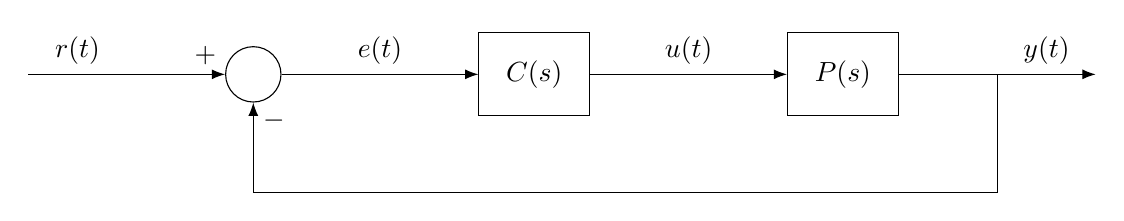
\begin{tikzpicture}[auto, node distance=2.5cm, >=Latex]

    % Place the nodes
    \node [input] (input) {};
    \node [sumstyle, right=of input] (sum) {}; % <-- Use new style 'sumstyle'
    \node [block, right=of sum] (controller) {$C(s)$};
    \node [block, right=of controller] (plant) {$P(s)$};
    \node [output, right=of plant] (output) {};

    % Draw the arrows and label them
    \draw [->] (input) -- node[near start] {$r(t)$} node[pos=0.9] {+} (sum);
    \draw [->] (sum) -- node {$e(t)$} (controller);
    \draw [->] (controller) -- node {$u(t)$} (plant);
    
    % Draw the output line AND create an invisible coordinate 'takeoff' halfway
    \draw [->] (plant) -- node[near end] {$y(t)$} (output) coordinate[pos=0.5] (takeoff);
    
    % Draw the feedback loop: Start at (takeoff), go down, then left, then up
    \draw [->] (takeoff) -- ++(0,-1.5) -| (sum.south) node[pos=0.9, right] {$-$};

    \end{tikzpicture}
    \caption{The block diagram of a generalized feedback control loop. $r(t)$ represents the desired value, $e(t)$ represents the error, and $y(t)$ represents the measured value. $C(s)$ represents the controller and $P(s)$ represents the process. }
    \label{fig:placeholder}
\end{figure}

The focus of control theory is on $u(t)$. One of the most prevalent control strategy is the use of Proportional, Integral, Derivative Controller or PID controller. These three terms was first introduced by Nicolas Minorsky in 1922s when he observed the action of helsman when navigating a ship.

The PID theory can be written as below:

\begin{equation}
     \\ u(t) = K_p e(t) + K_i \int\ e(\tau)d\tau + K_d \frac{de(t)}{dt}
\end{equation}

where $K_p  e(t)$ is the proportional terms which reacts to the present error, $K_i \int$ is the integral term which reacts to the accumulated historical error, and $K_d \frac{de(t)}{dt}$ is the derivative terms which reacts to the predicted error.

The PID control theory relies upon sensor measurement for the control action. The better the sensor is, the better the control action. However, most of PID control strategy applies in isolated control environment. Where in fact, industrial control itself is vast, and consist of multiple interconnected systems. This exact limitation, the gap between isolated PID loops and the interconnected reality of a plant, is what led to the development of Advanced Process Control (APC). 

While multiple PID controllers can be used, they often "fight" each other in a complex MIMO (Multiple-Input, Multiple-Output) system, leading to oscillations and suboptimal performance. This is where Model Predictive Control (MPC), a cornerstone of APC, provides a solution. Instead of being "blind," an MPC controller is built on a mathematical model of the process, such as a state-space model $y_{k+1} = f(y_k, u_k)$, which describes how the current state ($y_k$) and control action ($u_k$) influence the next state ($y_{k+1}$). 

This model allows the controller to predict the future behavior of the entire system over a "prediction horizon." At each time step, MPC solves an online optimization problem to find the best sequence of future control moves that will minimize a defined "cost function," which typically balances the goals of tracking the setpoint and minimizing control effort. This allows it to manage multiple variables simultaneously, anticipate cross-couplings, and find the optimal control strategy for the entire plant

MPC has been a robust control strategy for industrial control. However, it does have a few limitations and research gaps. Traditional MPC, which often relies on linear models, struggles to handle highly nonlinear or chaotic dynamic systems. This has led researchers to combine artificial intelligence with control theory, making the use of machine learning and neural networks more prevalent in process control. Therefore, there is a significant research opportunity to develop hybrid controllers. These controllers would replace the traditional linear model inside an MPC with a more powerful, data-driven model—such as a neural network—that can accurately capture the complex, nonlinear dynamics of the plant. This creates a clear research gap for models that are not only accurate but also computationally efficient and stable enough to be used in a real-time control loop

\begin{longtable}{ 
    >{\RaggedRight}p{4 cm} 
    >{\RaggedRight}p{2 cm} 
    >{\RaggedRight}p{4.5 cm} 
    >{\RaggedRight}p{4.5 cm} 
}
    
    % --- UPDATED TABLE HEADERS ---
    \toprule
    \textbf{Title} &
    \textbf{Author(s) \& Year} & 
    \textbf{Key Findings / Contributions} & 
    \textbf{Limitations \& Research Gaps} \\
    \midrule
    \endhead
    
    % --- TABLE FOOTER ---
    \bottomrule
    \endfoot
    
    % --- YOUR CONTENT GOES HERE ---
    
    % --- ROW 1 (REFORMATTED) ---
    Liquid Time Constant Networks &
    Hasani, R., et al. (2021) & 
    1. Demonstrates higher stability than standard RNNs. \newline
    2. Achieves higher accuracy compared to RNN, LSTM, and Latent ODEs. \newline
    3. Proposed as a robust framework for dynamic control systems. & 
    1. High memory and computational overhead during training. \newline
    2. Performance is dependent on the choice of ODE solver. \newline
    3. Possesses unexplored inherent causality (requires embedding physical laws). \newline
    4. Potential long-term dependency issues (vanishing gradient). \newline
    5. Numerical complexity and solver-dependency. \\
    \midrule
    
    % --- ROW 2 (REFORMATTED) ---
    Robust flight navigation out of distribution with liquid neural networks &
    Chahine, M., et al. (2023) &
    1. Achieves superior out-of-distribution (OOD) performance. \newline
    2. Demonstrates high robustness to perturbations. \newline
    3. Validates LNNs as a strong candidate for robust drone navigation. &
    1. Relies heavily on data augmentation for perception (could be replaced by embedded physical constraints). \newline
    2. Scope is limited to single-objective imitation learning. \newline
    3. Applicability to multi-objective scenarios is unexplored. \newline
    4. Causality is learned implicitly, not engineered; latent causal links cannot be explicitly utilized. \\
    \midrule

    % --- ROW 3 (REFORMATTED) ---
    Liquid Structural State Space Models &
    Hasani, R., et al. (2022) &
    1. Solves long-term dependency issues. \newline
    2. Achieves SOTA performance on long-range arena benchmarks. \newline
    3. Introduces a new mathematical method to approximate ODEs, removing the need for an advanced solver. &
    1. Limited to single-objective optimization. \newline
    2. High computational overhead, slightly exceeding standard S4 models. \newline
    3. Causal properties are not discussed. \newline
    4. Application to multi-objective environments is unexplored. \\
    \midrule

    LNN-PINN: A Unified Physics-Only Training Framework with Liquid Residual Blocks &
    Tao, Z., et al. (2025) &
    1. Achieves higher accuracy on complex systems compared to standard PINNs. \newline
    2. Leverages LNN's inherent ability to capture dynamic temporal data. \newline
    3. Uses LNN's gating parameters to control state information flow. &
    1. The framework remains deterministic and supervised. \newline
    2. Not applicable to multi-objective environments. \newline
    3. Primarily resolves PINN limitations; reciprocal benefits to the LNN architecture are not investigated. \\
    \midrule

    Dynamic Causal Modelling &
    Friston, K., et al. (2003) &
    1. Serves as the original inspiration for Liquid Time Constant Networks (LCTNs). \newline
    2. Provides a stable, probabilistic (Bayesian) framework for modeling connectivity in dynamic systems. \newline
    3. Demonstrates high robustness to noise and timing errors. \newline
    4. Reduces dynamic systems into three interpretable components: input-to-state, state-to-state, and modulatory parameters. \newline
    5. Decomposes non-dynamic elements into a bilinear approximation. &
    1. Heavy reliance on accurate priors, a requirement of its Bayesian approximation methods. \newline
    2. The original framework is modeled using a single state variable. \newline
    3. Highlights a key research question: Why LCTNs, inspired by DCM, abandoned the probabilistic Bayesian framework (potentially to model deterministic systems). \\
    \midrule


    Robust temporal knowledge inference via pathway snapshots with liquid neural network &
    Han, P., et al. (2025) &
    1. Achieves high performance in causal pathway prediction (e.g., disease evolution), outperforming Reinforcement Learning. \newline
    2. Maintains a low parameter count. \newline
    3. Models dynamic causal pathways by enriching static pathway snapshots with temporal data, using a multi-modal graph (semantic + relationship) and an LTC network. &
    1. Suffers from numerical stability constraints due to ODE solver dependency (e.g., Runge-Kutta). \newline
    2. Still exhibits issues with long-term dependencies. \newline
    3. Relies on predetermined static constraints to guide the network. \newline
    4. Key Gap: Synergizing the causal interpretation of LTCs with architectures that handle long-term dependencies (like Liquid S4). \newline
    5. Key Gap: Addressing the inherent numerical stability issues of the ODE-based approach. \\
    \midrule

    Causal Navigation by Continuous Time Neural Networks &
    Vorbach, C., et al. (2021) &
    1. Demonstrates true causal properties in continuous-time NNs, arguing that standard Neural ODEs lack this. \newline
    2. Achieves high performance and robustness in closed-loop systems (e.g., visual navigation). \newline
    3. Introduces Neural Circuit Policies (NCPs): sparse, LTC-based networks proposed as dynamic causal models. \newline
    4. Theorizes that Differential Equations inherently form causal structures. &
    1. Suffers from high numerical complexity during training. \newline
    2. Still exhibits issues with domain shift. \newline
    3. Vulnerable to long-term dependency issues (a limitation Liquid S4 may address). \newline
    4. Key Gap: Need for a hybrid model to address long-term dependencies, particularly when the temporal horizon is known. \\
    \midrule

        % --- NEW ROW ADDED ---
    Hybrid transformer model with liquid neural networks and learnable encodings for buildings’ energy forecasting &
    Antonesi, G., et al. (2025) &
    1. Outperforms Transformer, LSTM, and RNN benchmarks in energy forecasting accuracy. \newline
    2. Novel architecture integrates an LNN within the Transformer's self-attention mechanism to capture complex non-linear dynamics. \newline
    3. Employs a CNN and adaptive positional encodings for effective spatial-temporal feature extraction. \newline
    4. Demonstrates that LNNs can effectively complement Transformer models. &
    1. High computational resource demand, inherent to Transformer architectures. \newline
    2. Model struggles to account for abrupt changes in energy usage (e.g., transitional periods like morning/night). \newline
    3. Lacks benchmarking against other efficient Transformer variants (e.g., Informer). \\
    \midrule

    % --- NEW ROW ADDED ---
    Dynamic Sequential Neighbor Processing: A Liquid Neural Network-Inspired Framework for Enhanced Graph Neural Networks &
    Zhang, K., et al. (2025) &
    1. Outperforms standard GNNs by modeling static, unordered multi-order neighbors as a dynamic sequence. \newline
    2. Successfully captures temporal dynamics in graph structures. \newline
    3. Finds that sequential neighbor processing improves performance regardless of the temporal model used (LNN, LSTM, etc.). \newline
    4. Maintains low parameter count via the LNN. &
    1. Incurs high computational overhead, longer training times, and ODE-related complexity (uses a fused-ODE solver). \newline
    2. Key Gap: Performance degradation on some datasets, attributed to a "hypothesis mismatch" between the LNN's dynamic solution and the static complexity of the graph information. \\
    \midrule

    Closed-form continuous-time neural networks &
    Hasani, R., et al. (2022) &
    1. Introduces 'Closed-form continuous-time' (CfC) networks, an LCTN variant that removes ODE solver dependency. \newline
    2. Achieves a significant training speed-up (approx. 20\% of LNN time) by approximating the integral solution. \newline
    3. Maintains the expressivity and dynamic capabilities of LCTNs via a dynamic gate. &
    1. The approximation process may introduce information loss and causes a loss of mathematical invertibility/guarantees. \newline
    2. Still has potential for vanishing gradients, though this is partially mitigated by the gating mechanism. \newline
    3. Key Gap: Scalability of the architecture requires further investigation and improvement. \\
    \midrule

    A Tutorial on Energy Based Learning &
    LeCun, Y., et al. (2006) &
    1. Provides the first complete framework for Energy-Based Models (EBMs). \newline
    2. Proposes that the "energy" concept effectively captures latent variable connections. \newline
    3. Establishes that EBMs offer high normalization flexibility. \newline
    4. Identifies suitable loss functions (e.g., margin, negative log-likelihood) and the necessity of a contrastive training approach. &
    1. High computational expense, as training occurs over high-dimensional configurations. \newline
    2. Risk of model collapse (finding low-energy regions without penalizing high-energy ones) if not using a contrastive loss. \newline
    3. Potential for non-convex solutions in highly complex models. \newline
    4. Key Gap: Need for deeper theoretical understanding of loss functions. \newline
    5. Key Gap: Poor optimization and training efficiency. \newline
    6. Key Gap: Application to complex architectures and need for theoretical foundations for inference. \\
    \midrule

    How to train your energy-based models &
    Song, Y., \& Kingma, D. (2021) &
    1. Provides a comprehensive survey and analysis of EBM training methodologies (e.g., MCMC, Score Matching, NCE). \newline
    2. Establishes the theoretical connections and tradeoffs between these different objectives. \newline
    3. Highlights that most methods rely on sampling rather than training on the full dataset. &
    1. EBM training is computationally expensive and complex due to the intractable normalizing constant. \newline
    2. MCMC-based training requires careful hyperparameter tuning. \newline
    3. Score Matching methods are often not scalable. \newline
    4. Key Gap: Need for MCMC-free and/or more scalable training methods. \newline
    5. Key Gap: Potential to explore novel sampling guidance (e.g., physics-informed search). \\
    \midrule

    Improved contrastive divergence training of energy based models &
    Du, Y., et al. (2020) &
    1. Introduces a Contrastive Divergence (CD) training method for EBMs that relies on MCMC approximation, reducing sampling time. \newline
    2. Improves training stability by adding a KL divergence term to the loss. \newline
    3. Demonstrates that this CD method improves upon traditional EBMs and allows integration with modern deep learning components (tested on image generation). &
    1. The KL divergence term introduces additional computational overhead and a more complex backpropagation. \newline
    2. Performance relative to alternative training methods is not fully explored. \newline
    3. Key Gap: Need to test the method in domains beyond image generation. \newline
    4. Key Gap: Requires methods to reduce the KL divergence computational overhead. \newline
    5. Key Gap: Potential to integrate with amortized sampling to create hybrid models. \\
    \midrule

    Learning energy-based model with variational auto-encoder as amortized sampler &
    Xie, J., et al. (2021) &
    1. Proposes a novel unified framework that jointly trains an EBM and a VAE, addressing previous research gaps. \newline
    2. Uses the VAE as an "amortized sampler" to provide finite initialization for MCMC. \newline
    3. Achieves performance comparable to GANs while producing a meaningful latent space (good for interpretability). &
    1. Relies on finite sampling (approximation) with no mathematical guarantee of convergence. \newline
    2. The VAE is trained on a non-static objective, as the target changes with the EBM's sampling. \newline
    3. Key Gap: High complexity in balancing the two competing model objectives during joint training. \newline
    4. Key Gap: Need to solve the non-static objective problem and refine the sampling approximation. \\
    \midrule

    Flow contrastive estimation of energy-based models &
    Gao, R., et al. (2020) &
    1. Improves Contrastive Divergence (CD) training by incorporating a previously neglected KL divergence gradient term (L\textsubscript{kl}). \newline
    2. The full loss (L\textsubscript{cd} + L\textsubscript{kl}) simultaneously assigns low energy to real data while encouraging the MCMC sampler to be diverse and low-energy. \newline
    3. Demonstrates that including L\textsubscript{kl} and diverse sampling significantly improves EBM's generative capability. &
    1. The added L\textsubscript{kl} term introduces significant computational overhead. \newline
    2. High training complexity can prevent integration with other modern architectures. \newline
    3. Still reliant on MCMC sampling, which can be unstable or produce poor samples. \newline
    4. Key Gap: Need for improved computational efficiency of the KL term. \newline
    5. Key Gap: Scaling the framework to higher-dimensional data. \newline
    6. Key Gap: Application of this stable framework to new domains. \\
    \midrule

    Learning energy-based models by diffusion recovery likelihood &
    Gao, R., et al. (2020) &
    1. Introduces "diffusion recovery likelihood" to train EBMs on high-dimensional data (e.g., images). \newline
    2. Achieves SOTA, high-fidelity image generation by learning a sequence of conditional EBMs that "recover" clean samples from noisy ones. \newline
    3. Method allows for longer MCMC runs, improving tractability and partition function accuracy compared to MLE. &
    1. High computational cost associated with the diffusion and sampling processes. \newline
    2. Demonstrated limitations in scaling (e.g., tested up to 128x128 resolution). \newline
    3. Key Gap: The framework is limited to the image modality. \newline
    4. Key Gap: Application to other data types and improved scaling/efficiency are unexplored. \\
    \midrule

    Energy Transformer &
    Hoover, B., et al. (2023) &
    1. Introduces a novel EBM-Transformer hybrid, using an energy function, attention, and an associative (Hopfield) memory. \newline
    2. Inference is a continuous-time dynamic process that minimizes the global energy function. \newline
    3. Demonstrates strong performance across multiple domains (e.g., image completion, graph classification). \newline
    4. Achieves good memory efficiency, potentially due to the Hopfield network. &
    1. High computational cost of attention and issues with training stability. \newline
    2. The model can struggle to capture some global structures. \newline
    3. Key Gap: Aims to make static Transformers dynamic, but this introduces significant challenges. \newline
    4. Key Gap: High complexity and difficulty in designing the optimal global energy function. \\
    \midrule

    % --- NEW ROW ADDED ---
    Energy-Based Transformers are Scalable Learners and Thinkers &
    Gladstone, A., et al. (2025) &
    1. Introduces a scalable training paradigm for EBTs (similar to diffusion) that avoids the "curse of dimensionality." \newline
    2. Demonstrates superior performance over standard Transformers in bidirectional and continuous modalities. \newline
    3. Reports emergence of "System 2" thinking (reasoning) capabilities. \newline
    4. Successfully achieves three facets: dynamic computation allocation, uncertainty modeling, and prediction verification. \newline
    5. Training is framed as an optimization problem (minimizing a global energy function) using Langevin dynamics for exploration. &
    1. Suffers from training stability issues and high hyperparameter sensitivity. \newline
    2. Requires high computational resources. \newline
    3. Faces challenges with multimodal data distributions. \newline
    4. Key Gap: An autoregressive variant of the architecture was not successfully developed. \newline
    5. Key Gap: Further exploration of advanced MCMC / sampling methods is needed. \\
    \midrule

    Physics-informed neural networks: A deep learning framework for solving forward and inverse problems involving nonlinear partial differential equations &
    Raissi, M., et al. (2019) &
    1. Introduces the foundational "Physics-Informed Neural Networks" (PINNs) framework, a universal function approximator. \newline
    2. Successfully bridges deep learning and physics by incorporating a "physics loss" (PDE-based) with the standard "data loss." \newline
    3. Demonstrates superior accuracy in solving forward problems and success in data-driven discovery (inverse problems). &
    1. Does not aim to replace traditional computational methods but to complement them. \newline
    2. Original framework uses standard MLPs. \newline
    3. Key Gap: Lacks exploration into optimal neural network architectures (e.g., depth, width) suitable for PINNs. \newline
    4. Key Gap: Uncertainties in network design and comprehensive comparisons to traditional DL models are not fully explored. \\
    \midrule

    When and why PINNs fail to train: A neural tangent kernel perspective &
    Wang, S., et al. (2022) &
    1. Introduces the Neural Tangent Kernel (NTK) as a formal analysis tool to understand PINN training pathology. \newline
    2. Uses NTK eigenvalue analysis to diagnose training failure modes (e.g., stiffness). \newline
    3. Provides theoretical proof that PINNs converge to Gaussian processes (in the analyzed context). \newline
    4. Proposes an algorithmic solution (NTK-based weight calibration) to remedy training failure. &
    1. The theoretical proofs are limited to shallow networks (one hidden layer) and simple (linear 1D) PDEs. \newline
    2. The effectiveness of the proposed adaptive solution is not fully explored for all scenarios. \newline
    3. Key Gap: Requires generalization and expansion of the NTK analysis to deeper, more complex architectures and higher-dimensional, non-linear problems. \\
    \midrule

    Physics-informed neural networks for heat transfer problems &
    Cai, S., et al. (2021) &
    1. Successfully applies PINNs to complex heat transfer problems (e.g., Navier-Stokes, Stefan), especially where temperature data is scarce. \newline
    2. Solves ill-posed inverse problems that are difficult for traditional methods. \newline
    3. Introduces a novel and effective method for optimal sensor placement. \newline
    4. Accelerates the design space exploration process. &
    1. Training remains a non-convex optimization problem. \newline
    2. Demonstrates poor extrapolation accuracy outside of the training distribution. \newline
    3. Key Gap: Lacks established industrial-scale benchmarks for validation and comparison. \\
    \midrule

    Bayesian physics-informed neural networks for forward and inverse PDE problems with noisy data &
    Yang, L., et al. (2021) &
    1. Introduces a Bayesian PINN (B-PINN) framework, treating the problem probabilistically to mitigate noisy data and prevent overfitting. \newline
    2. Uses a Bayesian Neural Network (BNN) to form priors on unknown PDE terms. \newline
    3. Demonstrates higher accuracy, better noise handling, and effectiveness in solving inverse problems. \newline
    4. Requires Hamiltonian Monte Carlo (HMC) for the solution search space. &
    1. The HMC method incurs a very high computational cost. \newline
    2. The framework is limited by data size. \newline
    3. Key Gap: The proposed KL expansion for low-dimensional problems needs to be generalized and scaled to high-dimensional scenarios. \\
    \midrule

    An expert's guide to training physics-informed neural networks &
    Wang, S., et al. (2023) &
    1. Provides a comprehensive guide to PINN training, identifying key failure modes: spectral bias, unbalanced loss terms, and causality violations. \newline
    2. Proposes specific solutions: (a) Random Fourier Features for spectral bias, (b) NTK or gradient-based weighting for unbalanced loss, and (c) non-dimensionalization for variable scale disparity. \newline
    3. Suggests LNNs as a potential solution for difficulties in simulating long-term dynamics. &
    1. Highlights a significant lack of common, standardized benchmarks for PINN performance. \newline
    2. Causality violation in time-dependent PDEs is identified as a key challenge (which LNNs may solve). \newline
    3. Key Gap: Overall methodological advancements are still open for improvement. \\
    \midrule


    

\end{longtable}


% --- SECTION 3: METHODOLOGY ---
\section{Methodology}
The methodology section details the design of the hybrid architecture used in this study. It first addresses the Closed-form Continuous-time (CfC) network, explaining how its closed-form solution bypasses the computational bottleneck of iterative ODE solvers. The section then progresses to a feasibility assessment of the hybrid system, specifically detailing the training strategy employed to couple Energy-Based Models (EBMs) with LNNs. The results of this study are analyzed to determine the practical validity of the research hypothesis.

Building upon the feasibility confirmation, the chapter proceeds to the formal construction of the hybrid architecture, describing the integration of thermodynamic constraints within the CfC framework. Subsequently, the experimental workflow is defined, describing the end-to-end pipeline from data acquisition and preprocessing to model training and final evaluation metrics. The section concludes by presenting the research timeline, providing a chronological roadmap of the project milestones and the projected schedule for development and validation. This does also includes the resources and support required for the research.

\subsection{Closed Form Continuous Variant}
For the hybrid architecture, a more efficient variant of Liquid Neural Network (LNNs) is selected called Closed Form Continuous (CfC). Published and introduced in a paper by Hasani et al. the CfC variants of LNN is designed to remove one of the major limitations of LNNs, which is the requirements of ODE solver during training. 

ODE solver is putting high computational load to the LNNs. It makes the network less enticing to researcher despite it's efficiency and reduction in parameter size. Therefore, Hasani et al. aim to resolve this issues by approximating the LNNs ODEs into a closed form solution.

First, let's understand the current LNNs equation and why it requires ODE solver.

\begin{equation}
    \frac{dx(t)}{dt} = - [\frac{1}{\tau} + S(t,\theta)]x(t) + S(t,\theta)A.
\end{equation}

where $S(t,\theta)$ can be written as $f(x(t),I(t),\theta)$. For simplification, a single neuron without connection can be written as below,

\begin{equation}
    \frac{dx(t)}{dt} = - [w_t + f(I(t))]x(t) + f(I(t))
\end{equation}

This is called as initial value problem or IVP. To solve this equation, 



% --- SECTION 4: PROPOSED TIMELINE ---
\section{Proposed Timeline}
Provide a realistic schedule for your research. A table is the best way to show this. We are using a standard 'tabular' environment with \texttt{\\hline} for simplicity.

\begin{table}[htbp] % [htbp] lets LaTeX decide the best place for the table
    \centering
    \caption{Gantt Chart for Research Activities}
    \label{tab:timeline}
    \begin{tabular}{|l|l|} % The | adds vertical lines
        \hline % Top line of the table
        \textbf{Time Period} & \textbf{Task} \\
        \hline % Middle line
        Months 1-3         & Literature Review \& Finalizing Design \\
        Months 4-6         & Data Collection (Phase 1) \\
        Months 7-9         & Data Analysis (Phase 1) \\
        Months 10-12       & Data Collection (Phase 2) \\
        Months 13-15       & Final Data Analysis \\
        Months 16-18       & Writing Dissertation/Thesis \\
        \hline % Bottom line
    \end{tabular}
\end{table}


% --- 5. REFERENCES ---
% This is the final section. Because we cannot use external .bib files,
% we create the bibliography manually.
% The '{9}' tells LaTeX to make space for single-digit numbers (e.g., [1], [9]).
% If you have 10-99 references, use '{99}'.

\section*{References} % The * makes the section unnumbered
\begin{thebibliography}{9}

    % Each reference is a \bibitem with a unique key.
    % This key (e.g., 'key_paper_1') is what you use in the \cite{} command.
    
    \bibitem{key_paper_1}
    Author, A. N., \& Second-Author, B. (Year). Title of the journal article.
    \textit{Name of the Journal}, Volume(Issue), page-range.

    \bibitem{key_book_2}
    Writer, A. (Year). \textit{Title of the Book}. Publisher Name.
    
    \bibitem{your_next_source}
    ...and so on.

\end{thebibliography}


% --- 6. END OF DOCUMENT ---
\end{document}

